\chapter{Ziel und Funktion des Aufbaues}

Durch den Versuchsaufbau soll es möglich sein die Motorkennlinie eines Elektromotors nachzuweisen.
Hierfür muss

\begin{itemize}
    \item die Drehzahl gemessen,
    \item sowie durch Bremsen des Motors das Drehmoment ermittelt werden.
\end{itemize}

Die Drehzahlmessung erfolgt mittels eines IR-Sensors mit einer Läuferscheibe, deren Fläche halb schwarz, halb reflektierend ist.

\begin{figure}[H]
    \begin{center}
        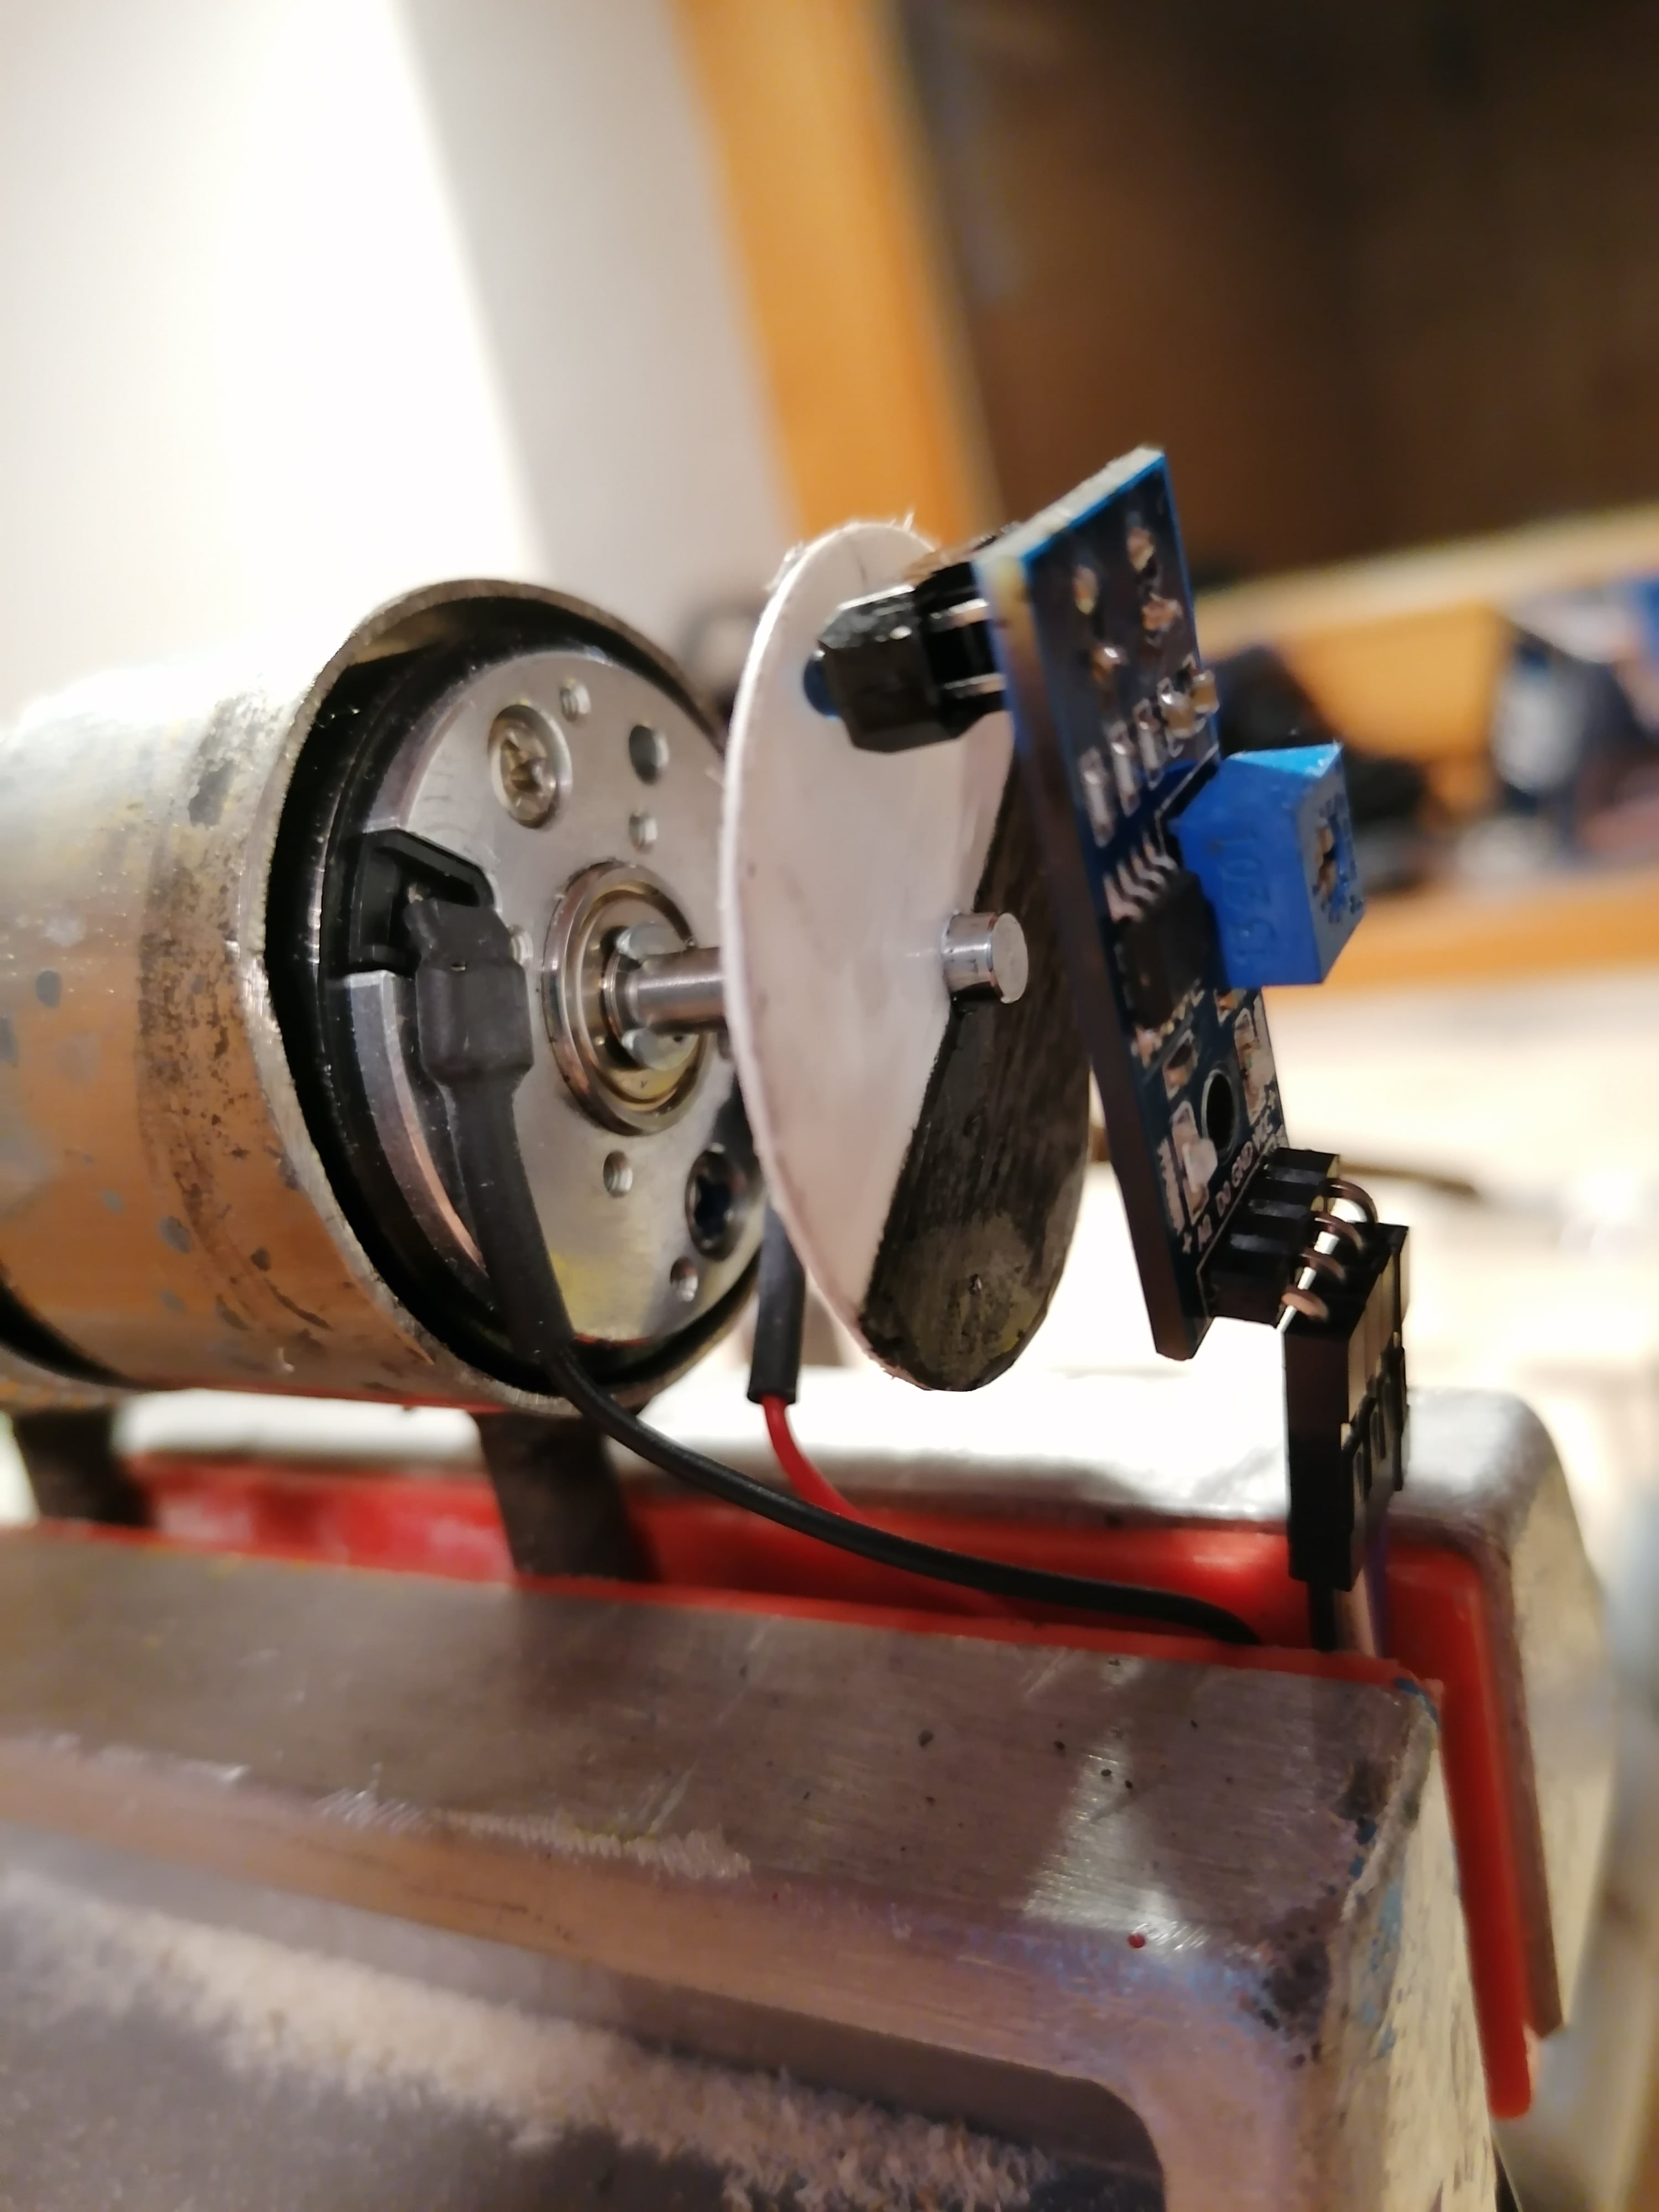
\includegraphics[width=0.3\textwidth]{drehzahl.jpg}
        \caption{Drehzahlmessung mittels IR-Sensor und Scheibe}
    \end{center}
\end{figure}

Die Drehmomentmessung erfolgt durch Verwendung eines mit dem Gehäuse des Motors verbundenen Armes, an dessem Ende sich eine Wägezelle befindet.

\begin{figure}[H]
    \begin{center}
        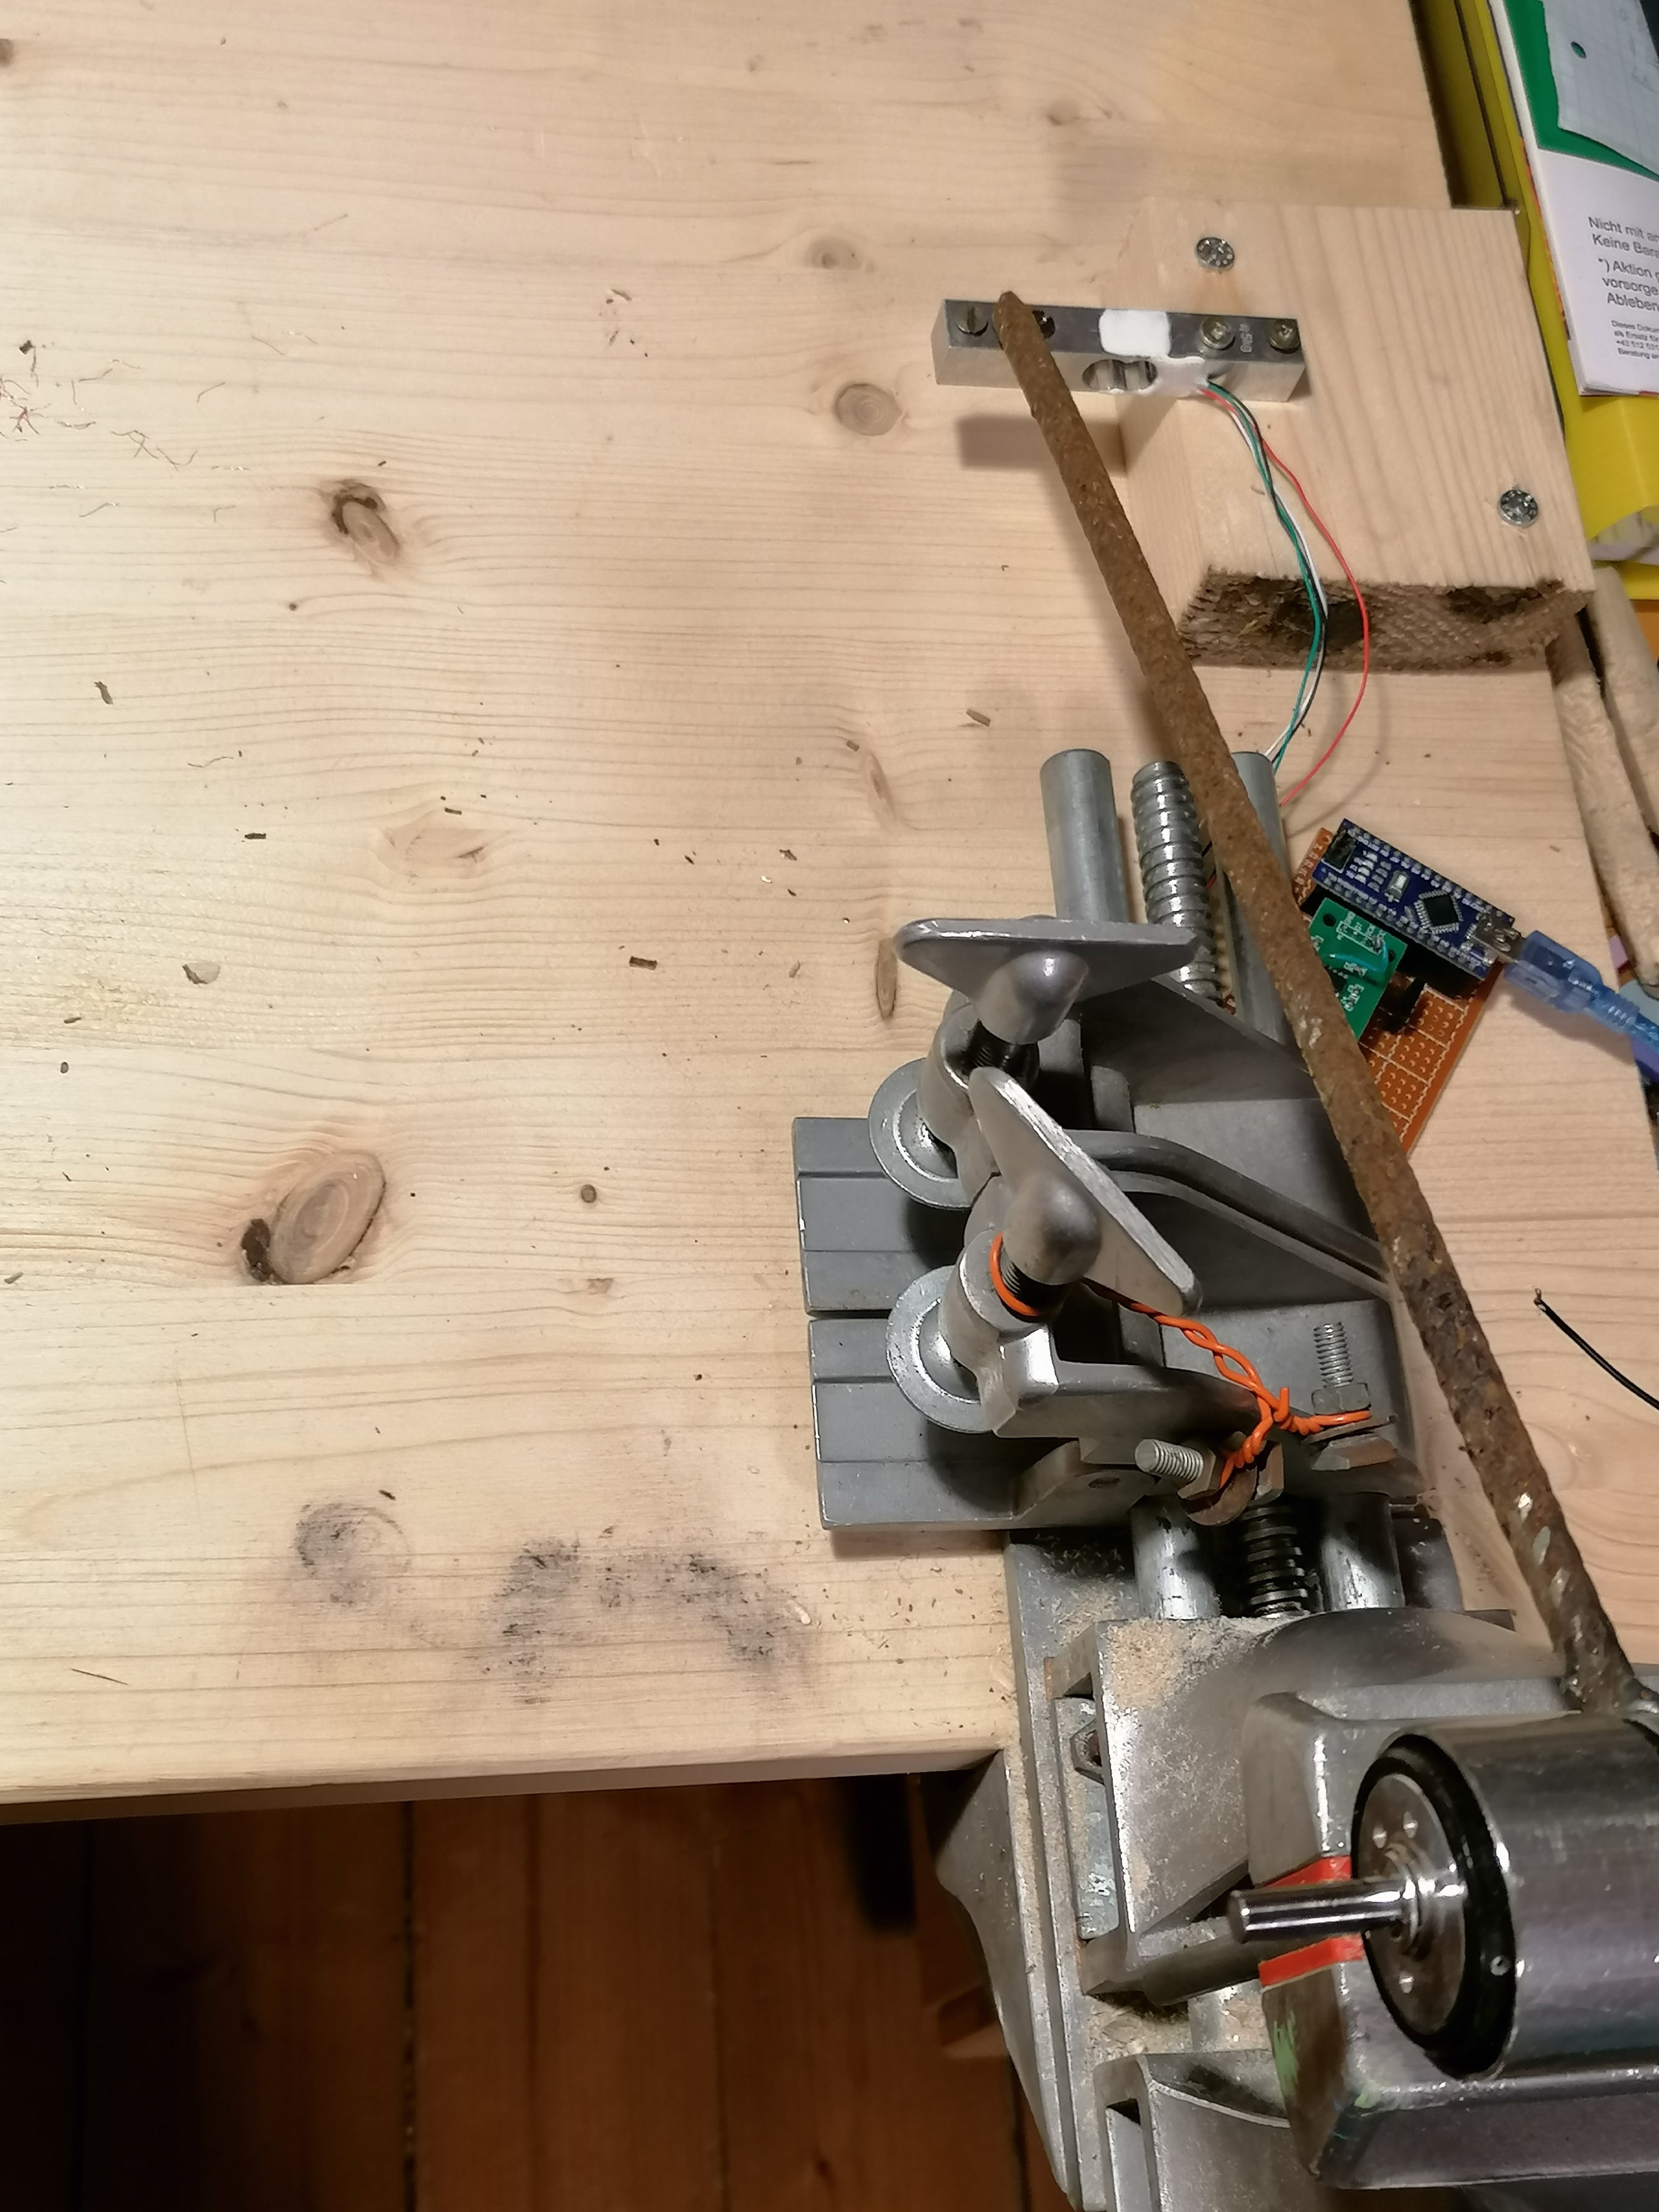
\includegraphics[width=0.3\textwidth]{drehmoment.jpg}
        \caption{Drehmomentmessung mit Arm und Wägezelle}
    \end{center}
\end{figure}

Weiters soll der Aufbau zur Durchführung einer Laborübung wie unter \hyperref[labuebung]{\textit{Teil 6}} verwendet werden.

Ursprünglich wurde dieser Versuchsaufbau für einen Motor dessen Gehäuse die Abmessungen (d x l) 36 x 72 hat angefertigt.
Jedoch ist dieses durch minimale Änderungen auch für die Verwendung mit Motoren ähnlicher Größe geeignet.
